\documentclass{beamer}
\usepackage[russian]{babel}
\usetheme{metropolis}

\usepackage{hyperref}

\usepackage{amsthm}
\usepackage{ulem}
\setbeamertemplate{theorems}[numbered]

\setbeamercolor{block title}{use=structure,fg=white,bg=gray!75!black}
\setbeamercolor{block body}{use=structure,fg=black,bg=gray!20!white}

\usepackage[T2A]{fontenc}
\usepackage[utf8]{inputenc}

\usepackage{hyphenat}
\usepackage{amsmath}
\usepackage{graphicx}

\AtBeginEnvironment{proof}{\renewcommand{\qedsymbol}{}}{}{}

\title{
Микроэкономика-I
}
\author{
Павел Андреянов, PhD
}

\begin{document}

\maketitle

\begin{frame}{План лекции}
\begin{itemize}
  \item Часть 1. Трейд + дорешать с прошлой лекции
  \item Часть 2. Больше КПВ. Повтор равновесия с производством.
\end{itemize}

Внимание, в это время, в прошлом году, я перестал регулярно перекладывать лекции в учебник, так что ориентируйтесь больше на слайды.
\end{frame}

\section{Парето всё (с консы)}
\begin{frame}{Парето всё}
На консультации я говорил о том, что максимизация взвешенной полезности это, вообще говоря, только достаточные условия, но не необходимые. Только когда все выпукло, непрерывно и строго монотонно вы получаете гарантированно (оба) Парето Фронта.
\begin{figure}[hbt]
\centering

\includegraphics[width=1 \textwidth]{pic1.png}
\end{figure}
Более того, если быть неаккуратным со знаком, то можно получить что-то вовсе неверное (см. последний пример на консультации с точками касания).
\end{frame}

\section{Трейд, пример 2 (с прошлой лекции)}

\begin{frame}{Пример 2}

Вернемся к примеру с прошлой лекции

Одна из двух стран (страна B) обладает абсолютным преимуществом в производстве всех товаров.
$$ F^A(X,Y) = X + Y/2 - 1 \leqslant 0, \quad F^B(X,Y) = X/4 + Y/2 - 1 \leqslant 0$$
Полезность Кобб Дуглас у обоих: $$U^i(x,y) = \log x + \log y, \quad i= {A,B}.$$
Напомню, что \alert{в трейде, у меня вектора $X, Y$ уже как бы содержат в себе начальные запасы.}
\end{frame}

\begin{frame}{Пример 2}
$$ F^A(X,Y) = X + Y/2 - 1 \leqslant 0, \quad F^B(X,Y) = X/4 + Y/2 - 1 \leqslant 0$$
\begin{figure}[hbt]
\centering
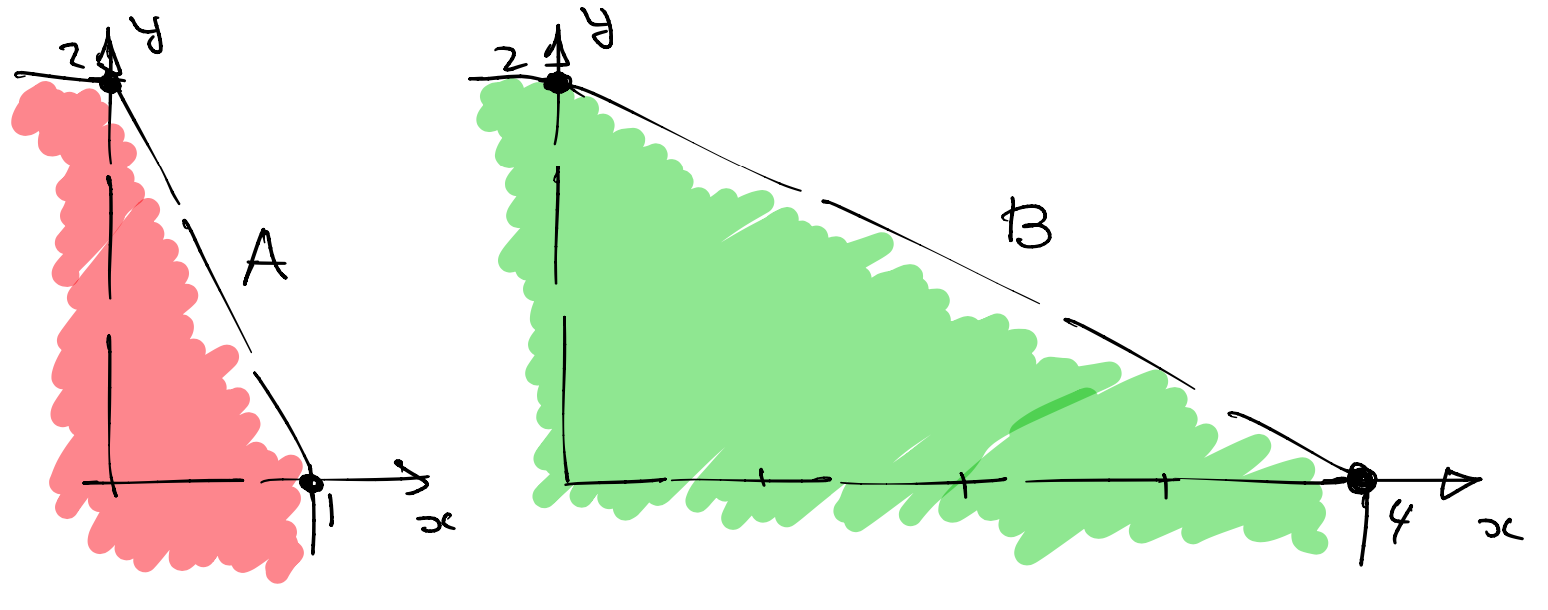
\includegraphics[width=1 \textwidth]{pic2.png}
\end{figure}
Пусть цена товара $x$ нормирована $p=1$, а товара $y$ равна $q$.
\end{frame}

\begin{frame}{Пример 2}
Найдем равновесие в автаркии для первой страны $A$. 

Опуская индекс страны, получаем УПП:
$$ \frac{U^{'}_x(x,y)}{U^{'}_y(x,y)} = \frac{1/x}{1/y} = \frac{1}{q} = \frac{1}{1/2} = \frac{F^{'}_X(X,Y)}{F^{'}_Y(X,Y)}$$
Моментально получаем что $q = 1/2$ и $y = 2x$.

Подставляя в соответствующие технологические границы, мы получаем координаты потребления $x = 1/2, y = 1$ и полезность $$U^{aut}_A = \log(1/2) + \log(1).$$

\end{frame}

\begin{frame}{Пример 2}
Найдем равновесие в автаркии для второй страны $B$. 

Опуская индекс страны, получаем УПП:
$$ \frac{U^{'}_x(x,y)}{U^{'}_y(x,y)} = \frac{1/x}{1/y} = \frac{1}{q} = \frac{1/4}{1/2} = \frac{F^{'}_X(X,Y)}{F^{'}_Y(X,Y)}$$
Моментально получаем что $q = 2$ и $y = x/2$.

Подставляя в соответствующие технологические границы, мы получаем координаты потребления $x = 2, y = 1$ и полезность $$U^{aut}_B = \log(2) + \log(1).$$

\end{frame}

\begin{frame}{Пример 2}
Найдем равновесие при международной торговле

Для этого надо понять, в каком из трех режимов работает экономика:

\begin{itemize}
  \item 1) $q = 1/2$, то есть страна $A$ не заметила разницы
  \item 2) $q = 2$, то есть страна $B$ не заметила разницы 
  \item 3) $q \in (1/2,2)$, то есть обе страны строго выиграли
\end{itemize}
Это легко визуализировать на совместной КПВ
\end{frame}

\begin{frame}{Пример 2}
\begin{figure}[hbt]
\centering
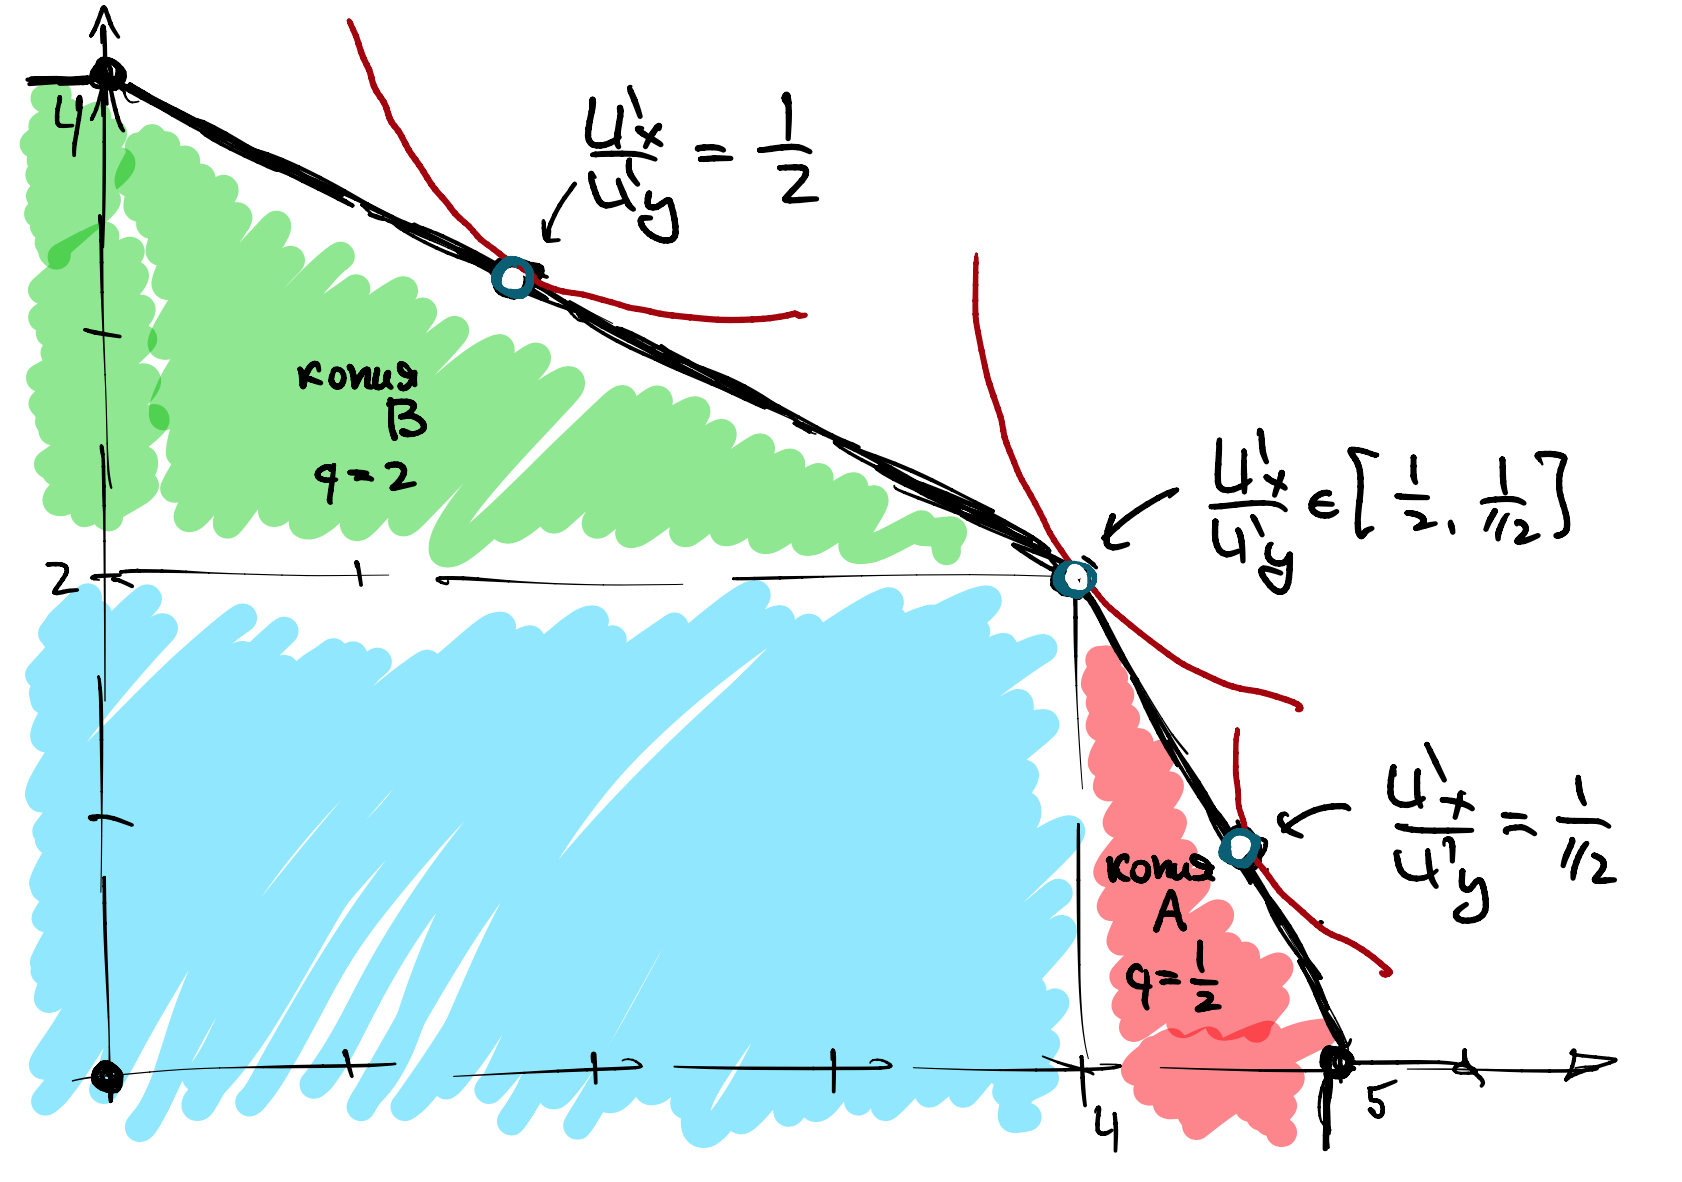
\includegraphics[width=1 \textwidth]{pic4.png}
\end{figure}
\end{frame}

\begin{frame}{Пример 2}
Далее будет перебор случаев, поэтому рекомендую завести табличку (даже несколько)

$$\begin{array}{c|c|c|c|c}
  \text{страна} & X & Y & x & y \\
  \hline
  A & & & &\\
  \hline
  B & & & &
\end{array}$$

\end{frame}

\section{Случай $q = 1/2$}

\begin{frame}{Пример 2}
Если $q = 1/2$ то мы находимся на <<правой арке>> КПВ
\begin{itemize}
  \item страна $A$ не заметила разницы между автаркией и международной торговлей, то есть $$x_A = 1/2, \ y_A = 1$$ но производить она может любую точку вдоль старой КПВ
  \item страна $B$ производит только первый товар, то есть
 $$X_B = 4, \ Y_B = 0$$
 но покупает какую-то внутреннюю точку
\end{itemize}
\end{frame}

\begin{frame}{Пример 2}
Мы разом заполнили половину таблички
$$\begin{array}{c|c|c|c|c}
  \text{страна} & X & Y & x & y \\
  \hline
  A & & & 1/2 & 1\\
  \hline
  B & 4 & 0 & &
\end{array}$$
\end{frame}

\begin{frame}{Пример 2}
Соответственно бюджет во второй стране равен $$4 p + 0 q = 4.$$ Спрос во второй стране выводится по формулам кобб-дугласа $$x_B = \frac{4}{2p} = 2, \ y_B = \frac{4}{2q} = 2/q = 4.$$
Мы заполнили табличку еще больше
$$\begin{array}{c|c|c|c|c}
  \text{страна} & X & Y & x & y \\
  \hline
  A & & & 1/2 & 1\\
  \hline
  B & 4 & 0 & 2 & 4
\end{array}$$
\end{frame}

\begin{frame}{Пример 2}
$$\begin{array}{c|c|c|c|c}
  \text{страна} & X & Y & x & y \\
  \hline
  A & & & 1/2 & 1\\
  \hline
  B & 4 & 0 & 2 & 4
\end{array}$$
Наконец, первой стране ничего не остается как произвести
\begin{align*}
	X_A & = x_A + x_B - X_B = 1/2 + 2 - 4 = -3/2\\
	Y_A & = y_A + y_B - Y_b = 1 + 4 - 0 = 5 
\end{align*}
Это явно противоречие, потому что \alert{в трейде, как правило, нельзя производить отрицательные количества товаров}, все товары потребительские. 

Однако, в домашке у вас будет специально по-другому. 
\end{frame}

\section{Случай $q = 2$}

\begin{frame}{Пример 2}
Если $q = 2$ то мы находимся на <<левой арке>> КПВ
\begin{itemize}
  \item страна $B$ не заметила разницы между автаркией и международной торговлей, то есть $$x_B = 2, \ y_B = 1$$
  \item страна $A$ производит только второй товар, то есть
 $$X_A = 0, \ Y_A = 2$$
 но покупает какую-то внутреннюю точку
\end{itemize}
\end{frame}

\begin{frame}{Пример 2}
Соответственно бюджет в первой стране равен $2q$. Спрос в первой стране выводится по формулам кобб-дугласа $$x_A = \frac{2q}{2p} = 2, \ y_A = \frac{2q}{2q} = 1 $$
Наконец, второй стране ничего не остается как произвести
\begin{align*}
	X_A & = x_a + x_b - X_B = 2 + 2 - 0 = 4\\
	Y_A & = y_a + y_b - Y_b = 1 + 1 - 2 = 0 
\end{align*}
Чудесным образом, это попадает в КПВ первой страны, УРА!!!
\end{frame}

\section{Случай $q \in (1/2,2)$}

\begin{frame}{Пример 2}
Если $q \in (1/2,2)$ то мы находимся на <<изломе>> КПВ
\begin{itemize}
  \item страна $A$ производит только второй товар, то есть
 $$X_A = 0, \ Y_A = 2$$
  \item страна $B$ производит только первый товар, то есть
 $$X_B = 4, \ Y_B = 0$$
\end{itemize}
При этом каждая страна покупает внутреннюю точку
\end{frame}

\begin{frame}{Пример 2}
Бюджет первой страны равен $2q$ а спрос соответственно
$$x_A = \frac{2q}{2p} = q, \quad y_A = \frac{2q}{2q} = 1 $$

Бюджет второй страны равен $4$ а спрос соответственно
$$x_B = \frac{4}{2p} = 2, \quad y_B = \frac{4}{2q} = 2/q $$

Приравнивая избыточный спрос $x$ к нулю получаем 
$$x_a + x_b - X_a - X_b = q + 2 - 0 - 4 = 0 \quad \Rightarrow \quad q = 2.$$

Формально, это противоречие, потому что $q \in (1/2,2)$.

\end{frame}

\section{Как перебирать случаи}

\begin{frame}{Пример 2}

Если вы не можете угадать режим решения с самого начала, рекомендую начать с <<излома>>, и если цена не попала в интервал перейти сразу к тому случаю, на который она пытается вам <<указать>>.

В данном случае, цена $q$ оказалась справа от интервала $(1/2,2)$ соответственно правильный режим это $q = 2$, или <<левая верхняя арка>> КПВ.

Но правильное решение тем не менее на изломе, так бывает если случайно сильно (не-)повезет с параметрами задачи.
\end{frame}

\section{Трейд, новый пример 3}

\begin{frame}{Пример 3}

Рассмотрим более сложный пример, с <<разными>> агентами.

Пусть у нас <<сферические>> технологии
$$ F^A(X,Y) = X^2 + Y^2 - 16 \leqslant 0, \quad F^B(X,Y) = X^2 + Y^2 - 9 \leqslant 0$$
Полезность Кобб Дуглас у первого: $$U^A(x,y) = \log x + \log y$$
и Леонтьев у второго $$U^B(x,y) = \min(x, y)$$
\end{frame}

\begin{frame}{Пример 3}
Найдем равновесие в автаркии для первой страны $A$. 

Опуская индекс страны, получаем УПП:
$$ \frac{U^{'}_x(x,y)}{U^{'}_y(x,y)} = \frac{1/x}{1/y} = \frac{p}{q} = \frac{2X}{2Y} = \frac{F^{'}_X(X,Y)}{F^{'}_Y(X,Y)}$$
Моментально получаем что $x = y$ и $p = q$.

Подставляя в соответствующие технологические границы, мы получаем координаты потребления $x = 4, y = 4$ и полезность $$U^{aut}_A = 2 \log 4.$$

\end{frame}

\begin{frame}{Пример 3}
Найдем равновесие в автаркии для второй страны $B$. 

Помним, что интересующее нас геометрическое место точек описывается уравнением
$$x = y$$

Подставляя в соответствующие технологические границы, мы получаем координаты потребления $x = y = \sqrt{9/2}$ и $$U^{aut}_B = \sqrt{9/2}$$
Цены можно, по прежнему, вытащить из фоков для фирмы
$$ \frac{p}{q} = \frac{2X}{2Y} = \frac{F^{'}_X(X,Y)}{F^{'}_Y(X,Y)}.$$
\end{frame}

\begin{frame}{Пример 3}
Попробуем общее равновесие.

Для построения совместного КПВ можно
\begin{itemize}
  \item воспользоваться геометрической интуицией
  \item построить руками через наклон
  \item max $X_{sum}$ при заданном $Y_{sum}$ или наоборот.
\end{itemize}
Последний подход мне кажется наиболее универсальным, но в этой задаче он немного тяжело решается...\end{frame}

\begin{frame}{Пример 3}
Но в этой задаче нам это даже и не поможет (потому что полезности разные), поэтому придется идти через избыточный спрос...

Пусть цены нормированы к $(1,q)$.
$$\begin{array}{c|c|c|c|c}
  \text{страна} & X & Y & x & y \\
  \hline
  A & ? & ? & ? &\\
  \hline
  B & ? & ? & ? &
\end{array}$$
Чтобы найти $q$ достаточно узнать все про товар $x$:
$$ x_A(q) + x_B(q) - X_A(q) - X_B(q) = 0$$
...немного подумав, убеждаемся что \alert{вычитать запасы тут не надо, потому что это трейд, тут запасы зашиты в $X,Y$}. Да и как их вычесть, если они в задаче даже не известны?
\end{frame}

\begin{frame}{Пример 3}
Пусть цены $(1,q)$ тогда производство определяется фоком
$$ \frac{1}{q} = \frac{2X}{2Y} = \frac{F^{'}_X(X,Y)}{F^{'}_Y(X,Y)}$$
подставляя в технологии получаем
$$X_A^2 = \frac{16}{1+q^2}, \quad Y_A^2 = \frac{16 q^2}{1+q^2}, \quad X_B^2 = \frac{9}{1+q^2}, \quad Y_B^2 = \frac{9 q^2}{1+q^2} $$
и бюджеты стран (внимание, корень сократился)
$$ I_a = 4 \sqrt{1+q^2}, \quad I_b = 3 \sqrt{1+q^2}$$
\end{frame}

\begin{frame}{Пример 3}
Теперь вспоминая кобдугласа
$$x_A = \frac{4 \sqrt{1+q^2}}{1}\frac{1}{2}, \quad y_A = \frac{4 \sqrt{1+q^2}}{q}\frac{1}{2}$$
и вспоминая леонтьева
$$x_B = y_B = \frac{3 \sqrt{1+q^2}}{1+q}$$
Осталось выписать избыточный спрос:
$$ E_x = \frac{4 \sqrt{1+q^2}}{2} + \frac{3 \sqrt{1+q^2}}{1+q} - \frac{4}{\sqrt{1+q^2}} - \frac{3}{\sqrt{1+q^2}} = 0$$
Тут есть один положительный корень $q=1$, потому что задача была нарочито составлена симметрично, а других таких нет (вольфрам), да их и не может быть по свойству валовости.
\end{frame}

\section{Вернемся к КПВ}

\begin{frame}{КПВ}
В прошлой задаче у вас были два КПВ:
$$ F^A(X,Y) = X^2 + Y^2 - 16 \leqslant 0, \quad F^B(X,Y) = X^2 + Y^2 - 9 \leqslant 0$$
и возможно вам потребовалось бы их объединить...

У вас на выбор 3 метода
\begin{itemize}
  \item воспользоваться геометрической интуицией
  \item построить руками через наклон
  \item max $X_{sum}$ при заданном $Y_{sum}$ или наоборот.
\end{itemize}
\end{frame}

\begin{frame}{КПВ}
Воспользоваться геометрической интуицией...
\begin{figure}[hbt]
\centering
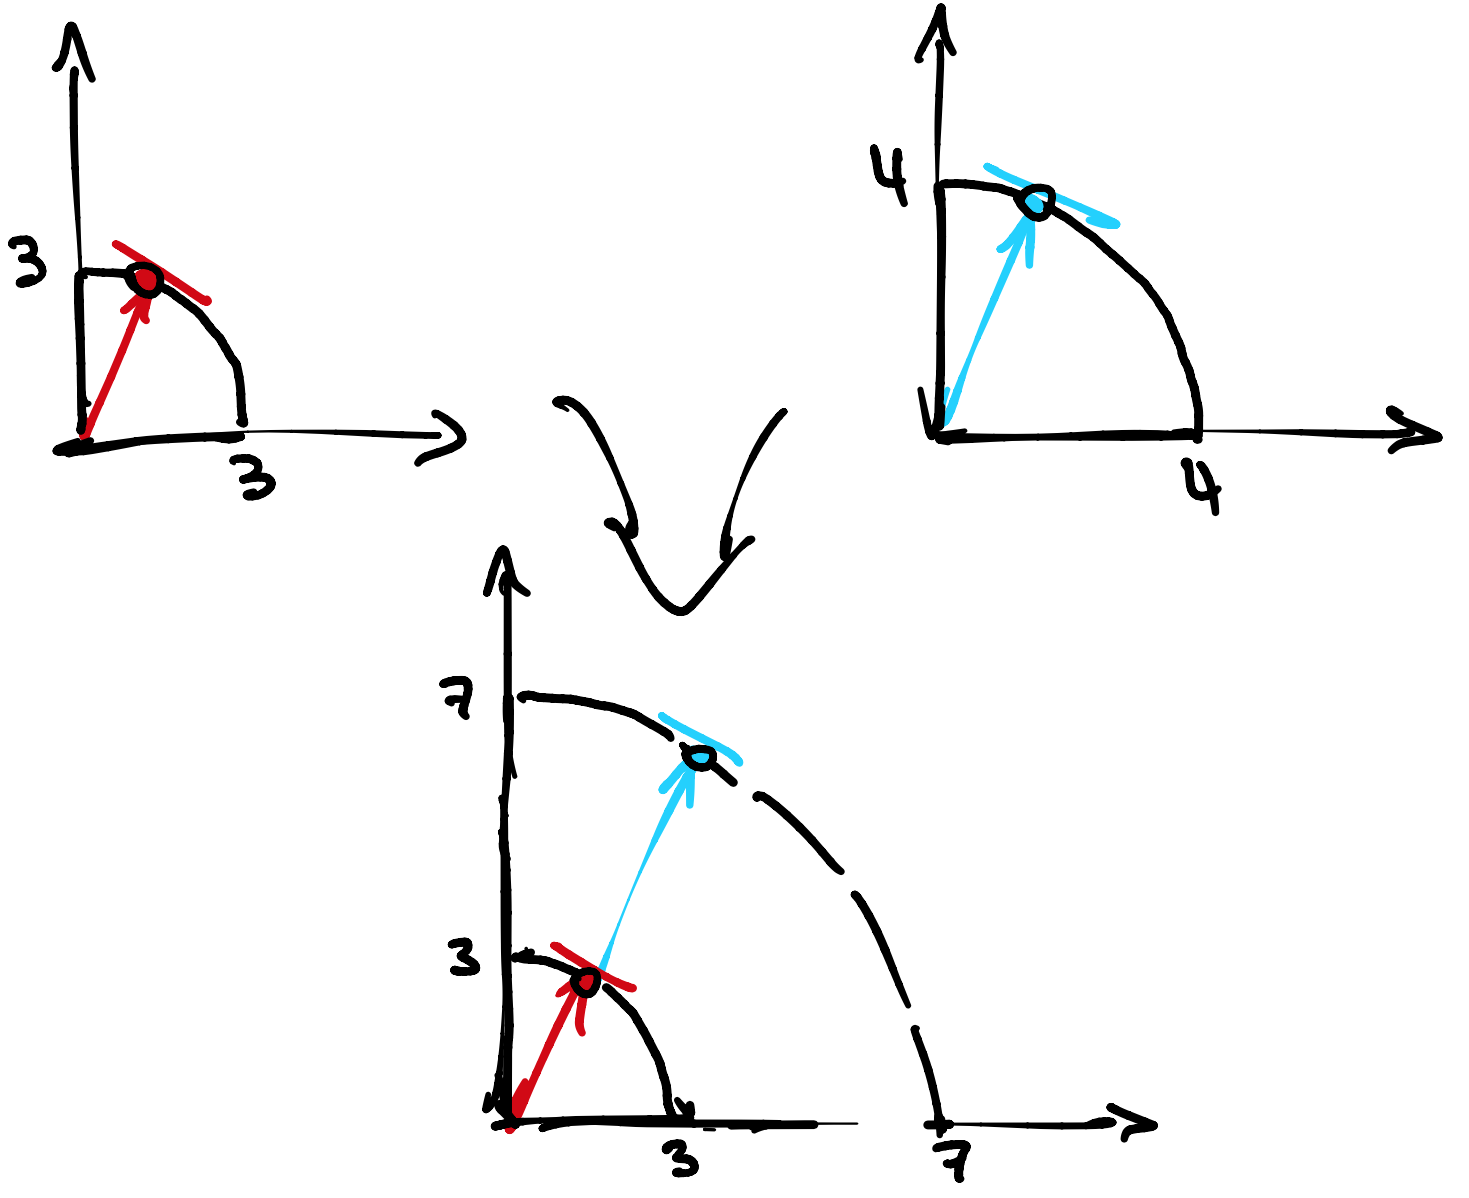
\includegraphics[width=.75 \textwidth]{pic5.png}
\end{figure}
\end{frame}

\begin{frame}{КПВ}
Построить руками через наклон вектора $\alpha$ (ему соответствует наклон касательной $\pi - \alpha$, который нас обычно интересует)
\begin{itemize}
  \item $X_a(\alpha) = 3 \cos \alpha, \quad Y_a(\alpha) = 3 \sin \alpha$
  \item $X_b(\alpha) = 4 \cos \alpha, \quad Y_b(\alpha) = 4 \sin \alpha$
\end{itemize}
Получается
$$ X_{sum}(\alpha) = 7 \cos \alpha, \quad Y_{sum}(\alpha) = 7 \sin \alpha$$
Это действительно уравнение окружности.
\end{frame}

\begin{frame}{КПВ}
Третий способ
$$ X_{sum} = X_A + X_B \to \max \quad s.t. \quad Y_{sum} = \sqrt{16-X_A^2} + \sqrt{9-X_B^2}$$
пишем фоки
$$ 1 + \lambda \frac{-2X_A}{2 \sqrt{16- X_A^2}} = 0, \quad 1 + \lambda \frac{-2X_B}{2 \sqrt{9- X_B^2}} = 0$$
делим, получаем
$$ \frac{X^2_A}{X^2_B} = \frac{16-X_A^2}{9-X_B^2} \quad \Rightarrow \quad 9 X_A^2 = 16 X_B^2$$
... и немного порешав уравнения ...
$$ X_A = \frac{4}{7} \sqrt{49-Y^2_{sum}}, \quad X_B = \frac{3}{7} \sqrt{49-Y^2_{sum}}$$ и наконец уравнение окружности $$X_{sum} = \sqrt{49-Y^2_{sum}}$$
\end{frame}

\section{Больше КПВ}

\begin{frame}{КПВ}
Геометрический подход самый результативный, на самом деле
\begin{figure}[hbt]
\centering
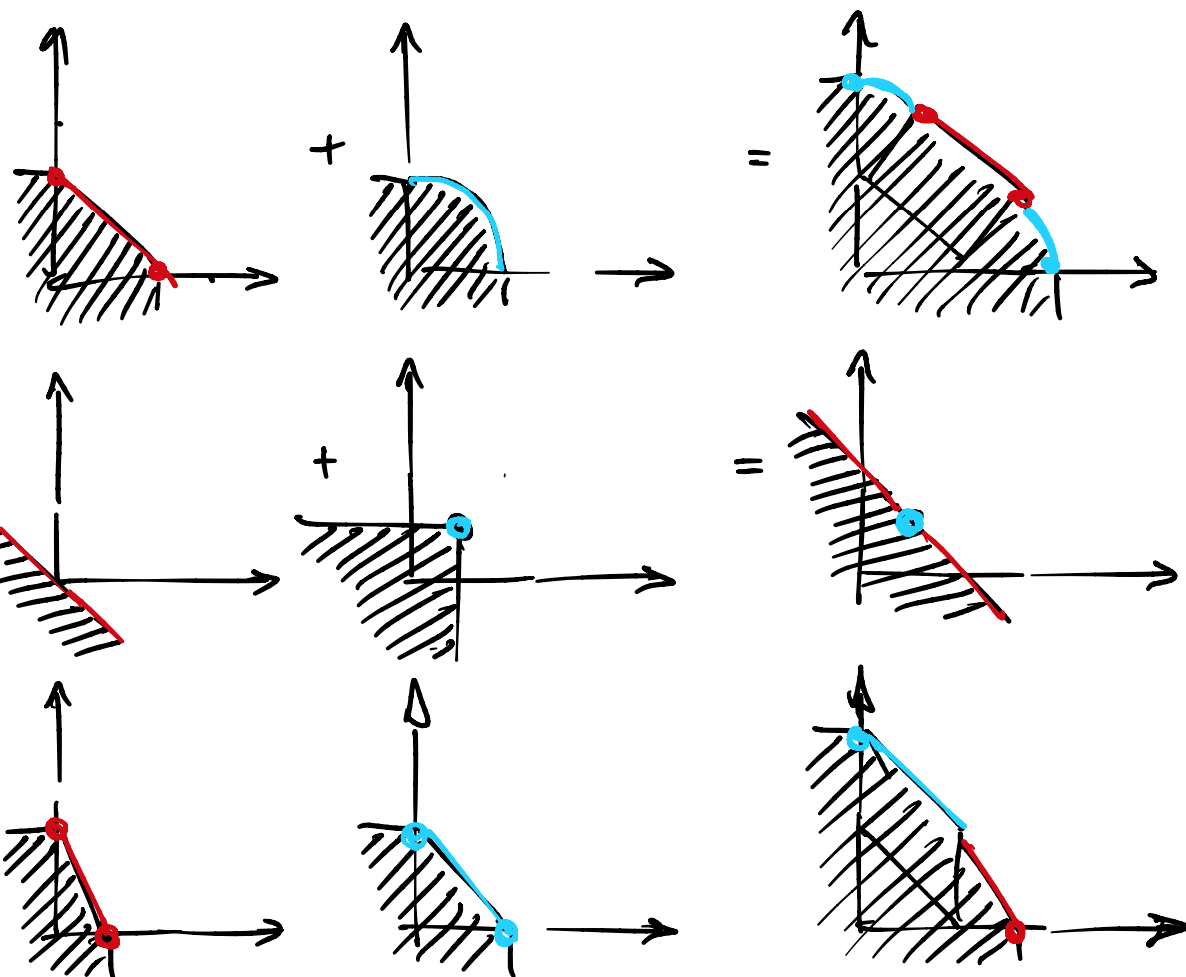
\includegraphics[width=.75 \textwidth]{pic6.png}
\end{figure}
\end{frame}

\section{Повтор РВ с производством}

\begin{frame}{Повтор РВ с производством}
У меня в планах решить 4 задачки
\begin{itemize}
  \item 1+1 (один агент одна фирма)
  \item 1+2 (один агент две фирмы)
  \item 2+1 (два агента одна фирма)
  \item 2+2 (два агента две фирмы) но точно не до конца
\end{itemize}
В каждой задаче надо выписать замкнутую систему уравнений, а также попытаться приравнять избыточный спрос к нулю.

Попробуем также поработать с табличкой, чтобы структурировать процесс решения.
\end{frame}

\section{1+1}

\begin{frame}{1+1}
Возьмем агента с (квазивогнутой) CES полезностью
$$ U(x,y) = \alpha \sqrt{x} + \sqrt{y}, \quad w = (2,3)$$
и, внимание, \alert{линейной} технологией
$$ F(X,Y) = X + Y \leqslant 0$$
Сходу сложно сказать, будет ли решение внутреннее, но мы всей душой в это верим и надеемся на собственную удачу.
\end{frame}

\begin{frame}{1+1}
Выпишем товарные равенства
$$ \ldots $$
Выпишем фоки 
$$ \ldots $$
Не забудем про эффективное производство
$$  \ldots $$
И закон Вальраса, но он последний, поэтому его не берем
$$ \ldots $$
и нормируем одну из цен, например, $p = 1$.

Должно быть пять уравнений на $(q,x,X,y,Y)$ неизвестных.
\end{frame}

\begin{frame}{1+1}
Выпишем товарные равенства
$$x = X + 2, \quad y = Y + 3$$
Выпишем фоки (тут совмещенные)
$$\frac{\alpha}{2\sqrt{x}} / \frac{1}{2\sqrt{y}} = p/q = 1/1$$
Не забудем про эффективное производство
$$ X + Y = 0$$
И закон Вальраса, но он последний, поэтому его не берем
$$ \xout{p x + q y = 2 p + 3 q}.$$

Должно быть пять уравнений на $(q,x,X,y,Y)$ неизвестных.

Вроде получилось.
\end{frame}

\begin{frame}{1+1}
Пытаться \alert{выписать избыточный спрос тут нет большого смысла}, потому что технология то линейная, \alert{цены, по сути известны}: $p=q=1$; поэтому придется решать систему.

Подставляем...
\begin{gather*}
\alpha \sqrt{y} = \sqrt{x}\\
x = X+ 2\\
y = \alert{Y} + 3\\
\alert{X+Y = 0}	
\end{gather*}
Совет: нелинейное уравнение лучше не трогать, решать начиная с линейных
\end{frame}
%
%\begin{frame}{1+1}
%Подставляем...
%\begin{gather*}
%\alpha \sqrt{y} = 2\sqrt{x}\\
%x = \alert{X}+ 2\\
%\alert{y = -X + 2}
%\end{gather*}
%\end{frame}
%
%\begin{frame}{1+1}
%Подставляем...
%\begin{gather*}
%\alpha \sqrt{y} = 2\sqrt{\alert{x}}\\
%\alert{x = 2 - y + 2}
%\end{gather*}
%
%\end{frame}
%\begin{frame}{1+1}
%Получается
%$$\alert{\alpha^2 y = 4 (2 - y + 2)}$$
%Или
%$$(\alpha^2 + 4) y = 16$$
%Или
%$$y = \frac{16}{\alpha^2 + 4} >0\quad \Rightarrow \quad x = 4 - y = \frac{4 \alpha^2}{\alpha^2 + 4}>0$$
%\alert{Решение внутреннее}, можно выдохнуть. 
%
%Цены равны (1,1), производство выводится элементарно через товарные равенства, значит равновесие найдено.
%
%\end{frame}

\section{1+2}

\begin{frame}{1+2}
Возьмем агента с полезностью кобб дуглас
$$ U(x,y) = \alpha \log x + \log y$$
и, двумя фирмами с технологиями
$$ F_{1}(X,Y) = X^2 + 2Y^2 \leqslant 1, \quad F_{2}(X,Y) = 2 X^2 + Y^2 \leqslant 1$$
Но фирмам запрещено производить отрицательные координаты, то есть, как в трейде, $X_{1}, Y_{1}, X_{2}, Y_{2} \geqslant 0$.
\end{frame}

\begin{frame}{1+2}
Поскольку тут фирма владеет всем, хотелось бы объединить КПВ, но он тут составной. Понадеемся на внутреннее решение и запишем условие эффективности производства:
$$ \frac{2X_1}{4Y_1} = \frac{p}{q}= \frac{4 X_2}{2 Y_2}$$
Запишем товарные равенства:
$$ x = X_1 + X_2, \quad y = Y_1 + Y_2$$
Наконец, запишем оптимальность потребления
$$ \frac{\alpha/x}{1/y} = \frac{p}{q}$$
Быстро сосчитали неизвестные $(q, x, y, X_1, Y_1, X_2, Y_2)$

Чего не хватает?
\end{frame}

\begin{frame}{1+2}

Вот такая система из 7 уравнений и 7 неизвестных

\begin{gather*}
	\frac{2X_1}{4Y_1} = \frac{1}{q}= \frac{4 X_2}{2 Y_2} = \frac{\alpha/x}{1/y}\\
	x = X_1 + X_2\\
	y = Y_1 + Y_2\\
	X_1^2 + 2Y_1^2 = 1\\
	2 X_2^2 + Y_2^2 = 1
\end{gather*}

Такое даже мне страшно решать, поэтому лучше выпишем избыточный спрос...

\end{frame}

\begin{frame}{1+2}
сначала придется сосчитать предложение 1ой фирмы
$$ X + q Y \to \max, \quad s.t. \quad X^2 + 2 Y^2 \leqslant 1$$
это довольно легко
$$ X + q \sqrt{\frac{1-X^2}{2}} \to \max$$
и тогда
$$ X^2_1 = \frac{2}{q^2 + 2}, \quad Y_1^2 = \frac{q^2/2}{q^2 + 2}$$
а прибыль
$$ \pi_1 = \frac{\sqrt{2} + q^2/\sqrt{2}}{\sqrt{q^2 + 2}} = \frac{\sqrt{q^2 + 2}}{\sqrt{2}}$$
\end{frame}

\begin{frame}{1+2}
теперь придется сосчитать предложение 2ой фирмы
$$ X + q Y \to \max, \quad s.t. \quad 2 X^2 + Y^2 \leqslant 1$$
это довольно легко
$$ X + q \sqrt{1-2 X^2} \to \max$$
и тогда
$$ X^2_2 = \frac{1}{2 + 4 q^2}, \quad Y^2_2 = \frac{4q^2}{2 + 4 q^2}$$
а прибыль
$$ \pi_2 = \frac{1 + 2 q^2}{\sqrt{2 + 4q^2}} = \frac{\sqrt{1+2q^2}}{\sqrt{2}}$$
\end{frame}

\begin{frame}{1+2}
В принципе, мы готовы выписать избыточный спрос
\begin{gather*} E_x(q) = x(q) - X_1(q) - X_2(q) = \\ = \frac{\alpha}{1+\alpha} \frac{1}{1}(\frac{\sqrt{q^2 + 2}}{\sqrt{2}} + \frac{\sqrt{1+2q^2}}{\sqrt{2}}) - \sqrt{\frac{2}{q^2 + 2}} - \sqrt{\frac{1}{2 + 4 q^2}}\end{gather*}
Можно убедиться, что при $\alpha = 1$ решение $q = 1$, что неудивительно, поскольку задача становится симметричной.

Для красоты, выпишу второй избыточный спрос.
\begin{gather*} E_y(q) = y(q) - Y_1(q) - Y_2(q) = \\ = \frac{1}{1+\alpha} \frac{1}{q}(\frac{\sqrt{q^2 + 2}}{\sqrt{2}} + \frac{\sqrt{1+2q^2}}{\sqrt{2}}) - \sqrt{\frac{q^2/2}{q^2 + 2}} - \sqrt{\frac{4q^2}{2 + 4 q^2}}\end{gather*}
Напоминаю, что тут как в трейде нет запасов.
\end{frame}

\section{2+1}

\begin{frame}{2+1}
Не так то легко придумать задачку так, чтобы она решилась.

Пусть есть две фирмы
$$U_a = min(2x, y), \quad w_a = (1,0)$$
$$U_b = min(x, 2y), \quad w_b = (0,1)$$
И завод
$$ F(X,Y) = \log(1-X) + \log(1-Y) - \log 2 \geqslant 0$$
которым они владеют поровну
\end{frame}

\begin{frame}{2+1}
Что делает фирма?
$$X + q Y \to max, \quad s.t. \quad \log(1-X) + \log(1-Y) - \log 2 \geqslant 0$$
Выпишем фоки
$$ 1 - \frac{\lambda}{1-X} = 0, \quad q - \frac{\lambda}{1-X} = 0$$
или
$$ 1 - X = \lambda, \quad 1-Y = \lambda / q$$
подставляя
$$ \log(\lambda) + \log (\lambda/q) - \log 2 = 0 \quad \Rightarrow \quad \lambda = \sqrt{2q}$$
отсюда находим
$$ X = 1 - \sqrt{2q}, \ Y = 1 - \sqrt{2}/\sqrt{q}, \ \pi = 1 + q - 2\sqrt{2q}$$
\end{frame}

\begin{frame}{2+1}
Агенты делят прибыль $\pi = 1 + q - 2\sqrt{2q}$ пополам, но у них еще деньги есть от продажи запасов, 1 у агента $a$, $q$ у агента $b$.

По формулам леонтьева
$$ x_a = \frac{1+\pi/2}{1+2q}, \ y_a = \frac{2+\pi}{1+2q}$$
$$ y_b = \frac{q+\pi/2}{2+q}, \ x_b = \frac{2q + \pi}{2+q}$$
тогда избыточный спрос
$$ E_x(q) = -1 +  \frac{1+\pi/2}{1+2q} + \frac{2q+\pi}{2+q} - (1-\sqrt{2q})$$
можно проверить что $q = 1$ подходит.
\end{frame}

\section{2+2}

\begin{frame}{2+2}
Пусть есть две фирмы
$$U_a = \log x + \log y, \quad w_a = (1,0)$$
$$U_b = \log x + \log y, \quad w_b = (0,1)$$
И заводы
$$ F_{\alpha}(X,Y) = \sqrt{1-X} - Y - 1 \geqslant 0$$
$$ F_{\beta}(X,Y) = \sqrt{1-X} - Y/2 - 1 \geqslant 0$$
причем $a$ владеет $\alpha$, $b$ владеет $\beta$.

Тут не очень сложно, поэтому выпишу избыточный спрос у доски, должно получиться квадратное уравнение.
\end{frame}

\end{document}
